\section*{Annexes} % Pas de numérotation
\phantomsection
\addcontentsline{toc}{section}{Annexes}
\appendix
\renewcommand\thefigure{\thesection.\arabic{figure}}
\setcounter{figure}{0}
\setcounter{section}{1}
%\setcounter{subsection}{1}


\subsection{\label{iot-lab}Distribution des nœuds FIT iot-lab}


\begin{figure}[ht!]
\centering
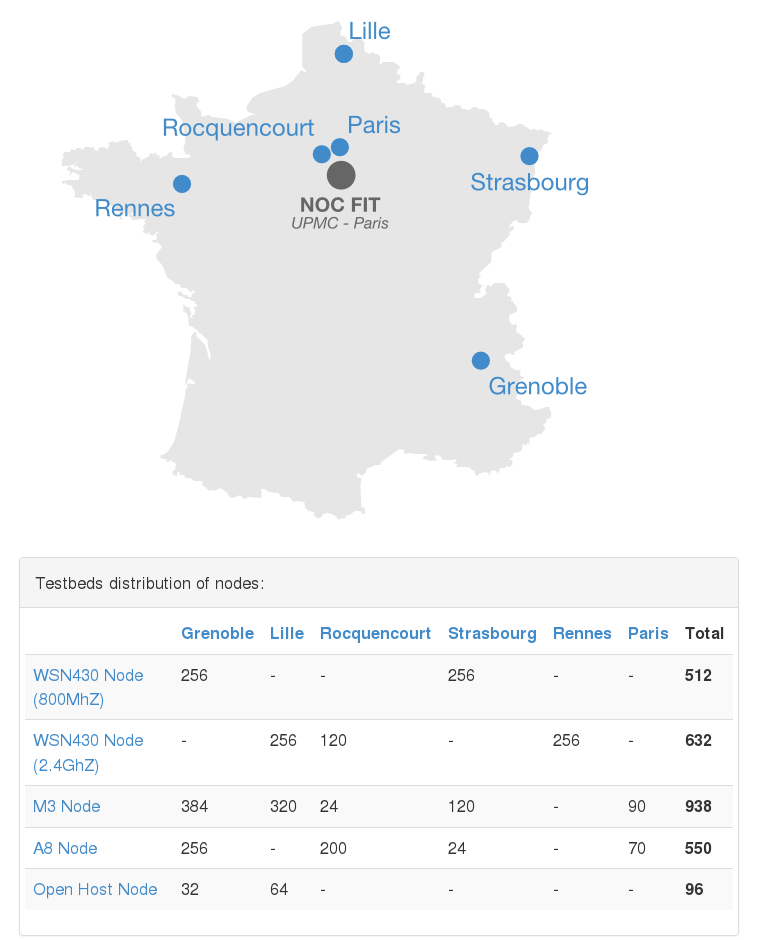
\includegraphics[scale=0.6]{images/iot-lab.png}
\caption{Source: https://www.iot-lab.info/deployment/}
\end{figure}

\subsection{\label{massif}Sortie de Massif}
\begin{figure}[ht!]
\centering
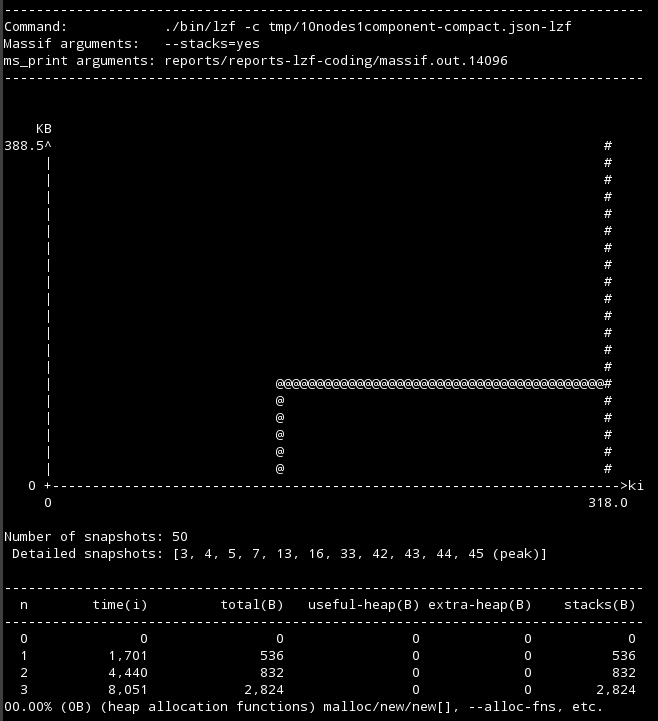
\includegraphics[scale=0.7]{images/msprint.png}
\caption{Exemple d'extrait de sortie de Massif, ici l'utilisation maximum de RAM est au snapshot 45 et est d'environ 400KB.}
\end{figure}

\begin{landscape}
\subsection{\label{comp-tabde}Compression de modèles}
\begin{figure}[ht!]
\centering
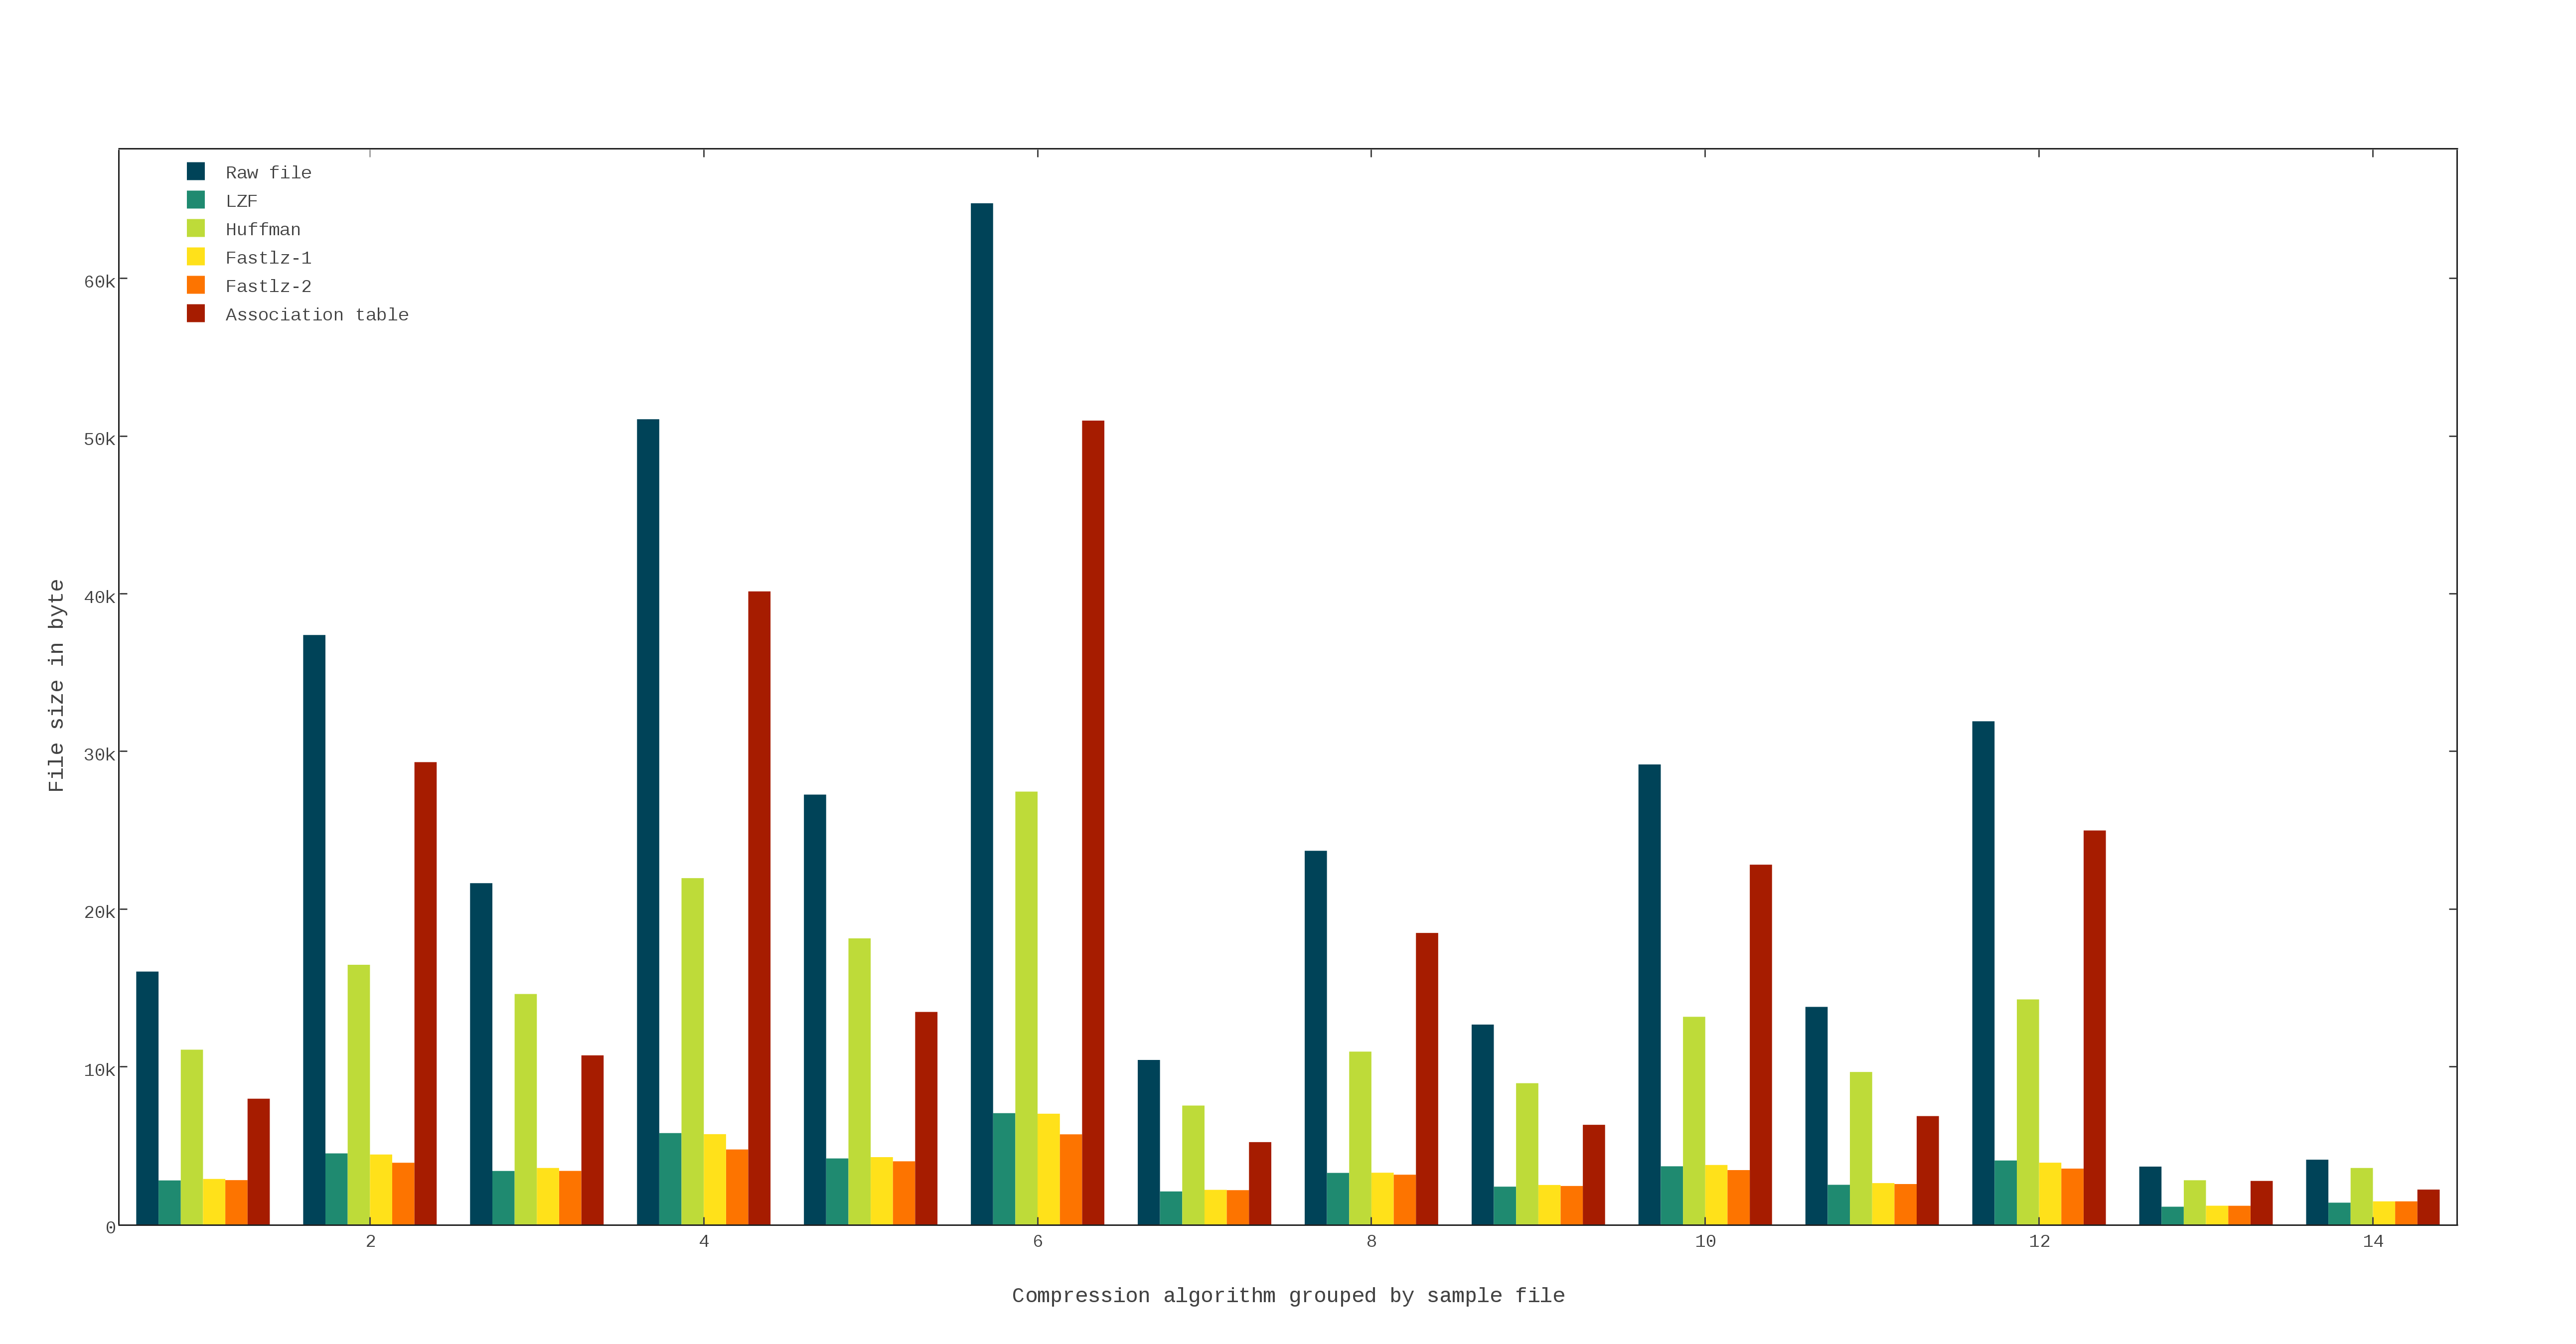
\includegraphics[scale=0.45]{images/compression.png}
\caption{Mesure de compression de modèles à l'aide de différents algorithmes}
\end{figure}
\end{landscape}

\begin{landscape}
\subsection{\label{kevoree-full-cd}Méta-modèle Kevoree}
\begin{figure}[ht!]
\centering
\fontsize{1mm}{4mm}\selectfont
\def\svgscale{0.28}
\input{images/kevoree-full-cd.pdf_tex}
\caption{Représentation du méta-modèle de Kevoree.}
\end{figure}
\end{landscape}